%
% einleitung.tex -- Beispiel-File für die Einleitung
%
% (c) 2020 Prof Dr Andreas Müller, Hochschule Rapperswil
%
% !TEX root = ../../buch.tex
% !TEX encoding = UTF-8
%
\section{Brownische Bewegung\label{brown:section:teil0}}
\rhead{Brownische Bewegung}

Als der Schottische Botaniker Robert Brown im Jahr 1827 in sein Mikroskop schaut, beobachtet er kleine Partikel von Pflanzenpollen in einer Flüssigkeit. Er bemerkt, dass sich die Teilchen scheinbar zufällig bewegen, obwohl scheinbar keine Kräfte auf die Teilchen einwirken. Eine Erklärung hatte Robert Brown zu diesem Zeitpunkt für das Verhalten noch nicht und notierte dass sich die Teilchen scheinbar zufällig und unregelmässig bewegen.

Es dauerte fast ein Jahrhundert, bis Albert Einstein diese Beobachtung auf ein solides theoretisches Fundament stellte und nutzbar machte. Er schloss darauf, dass dir unregelmässige Bewegung auf Kolisionen mit umgebenden Mölekühlen zurückzuführen ist, welche ständig in Bewegung sind. In seiner Theorie beschreibt er...

Die Brownische Bewegung kann relativ einfach simuliert werden mittels der Eueler-Maruyama-Methode. Diese wird häufig eingesetzt, um stochastische DIfferenzialgleichugnen zu simulieren.

\begin{equation}
	X_{n+1} = X_n + f(X_n,t_n) \Delta t + g(X_n,t_n) \Delta W_n
\end{equation}

Die Funktion f(X_n,t_n) beschreibt dabei den deterministischen Teil der SDE, im Kontext der Brown'schen Bewegung kann man es auch "drift nennen", welcher nicht nur von zufälligen Einflüssen bestimmt ist. Dies ist auch der Teil, der durch eine harmonische Analyse untersucht werden kann. Das Rauschen ("white noise"), welches hier mit g(X_n,t_n) beschrieben ist, enthält keine Information und kann somit nicht analysiert werden.

\Delta W beschreibt die Geschwindigkeit, mit welcher der stochastische Prozess ablaufen soll und W_n beschreibt den Wiener Prozess oder die Brownische Bewegung als Ganzes.

\begin{figure}
	\centering
	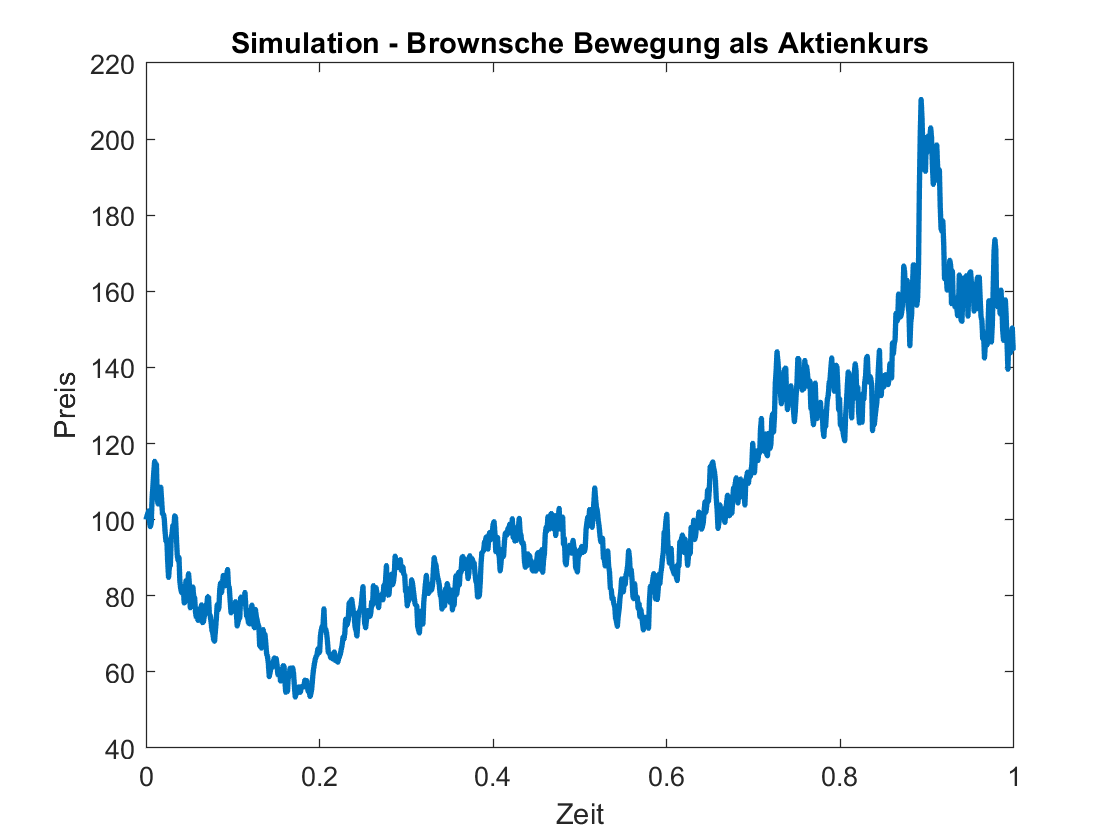
\includegraphics[width=0.7\linewidth]{papers/brown/images/Aktienkurs-als-Brownische-Bewegung_2.png}
	\caption{Simulation mittels der Eueler-Maruyama-Methode eines Aktienkurses}
\end{figure}

\begin{figure}
	\centering
	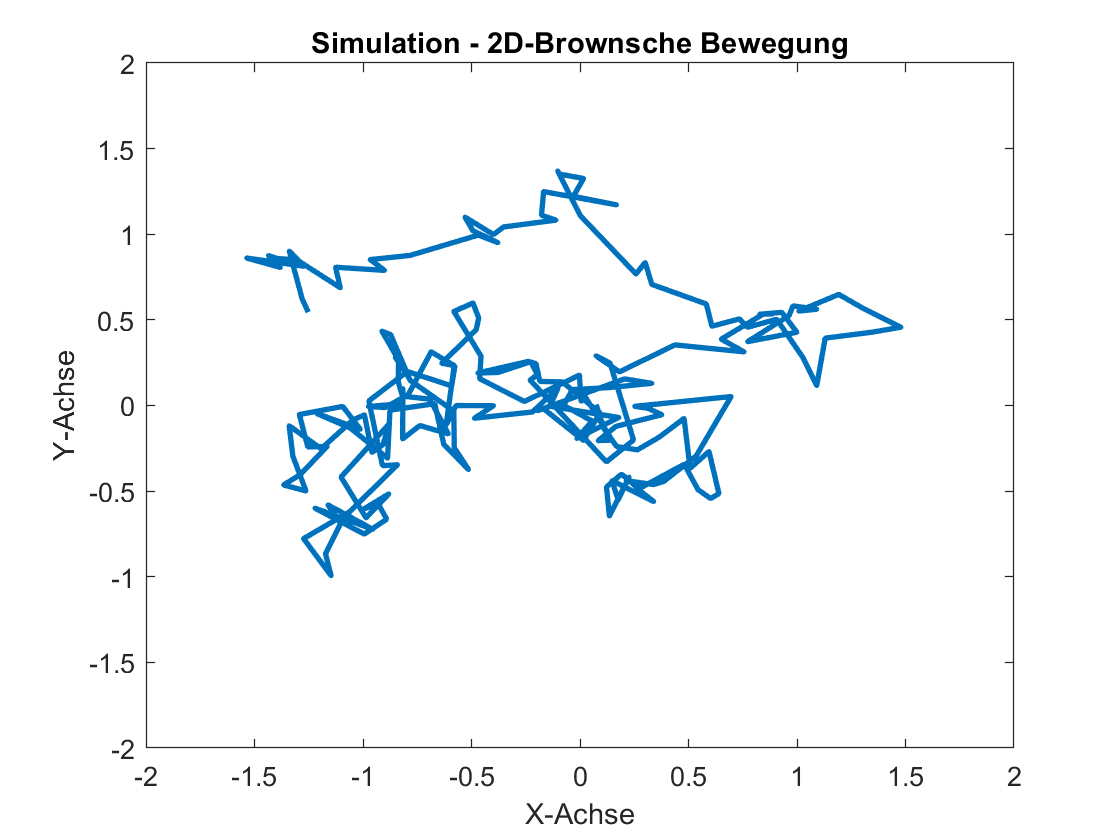
\includegraphics[width=0.7\linewidth]{papers/brown/images/Brownische-Bewegung-Simuliert_2.png}
	\caption{Simulation mittels der Eueler-Maruyama-Methode der Brown'schen Bewegung eines Teilchens}
\end{figure}


\begin{figure}
	\centering
	\begin{minipage}{0.45\textwidth}
		\centering
		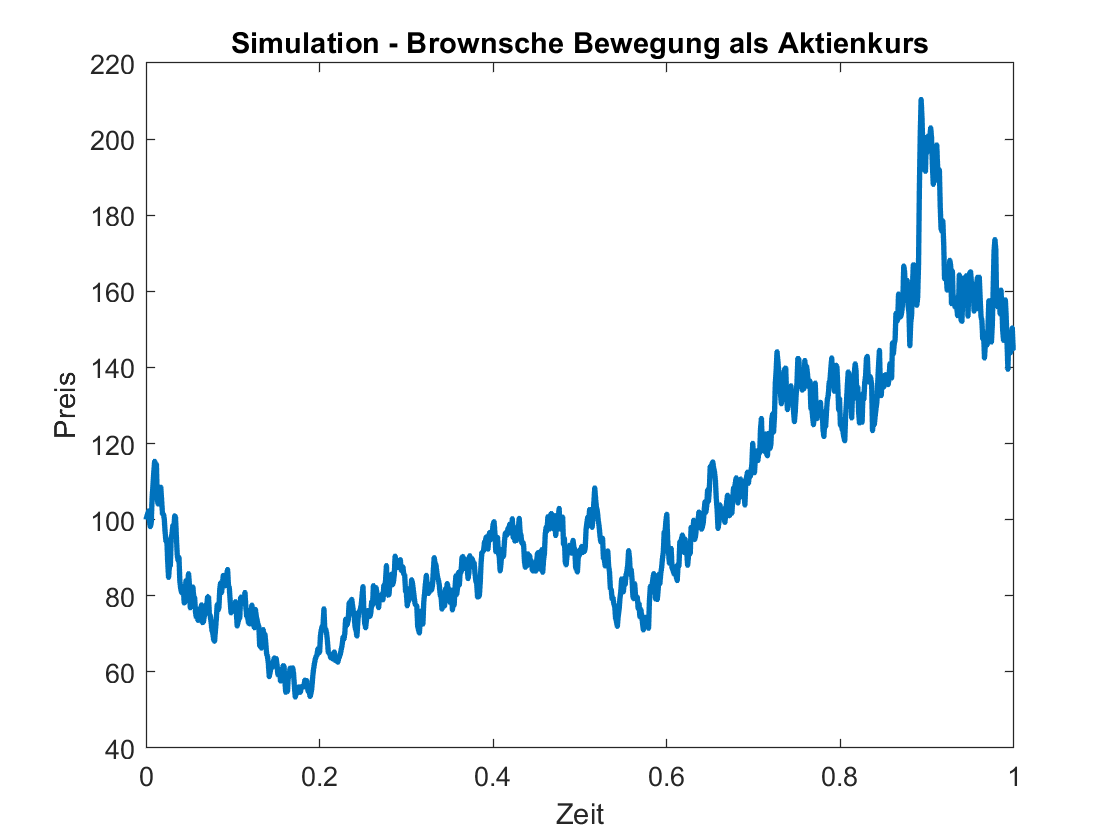
\includegraphics[width=\linewidth]{papers/brown/images/Aktienkurs-als-Brownische-Bewegung_2.png}
		\caption{First subfigure}
	\end{minipage}
	\hspace{0.05\linewidth}
	\begin{minipage}{0.45\textwidth}
		\centering
		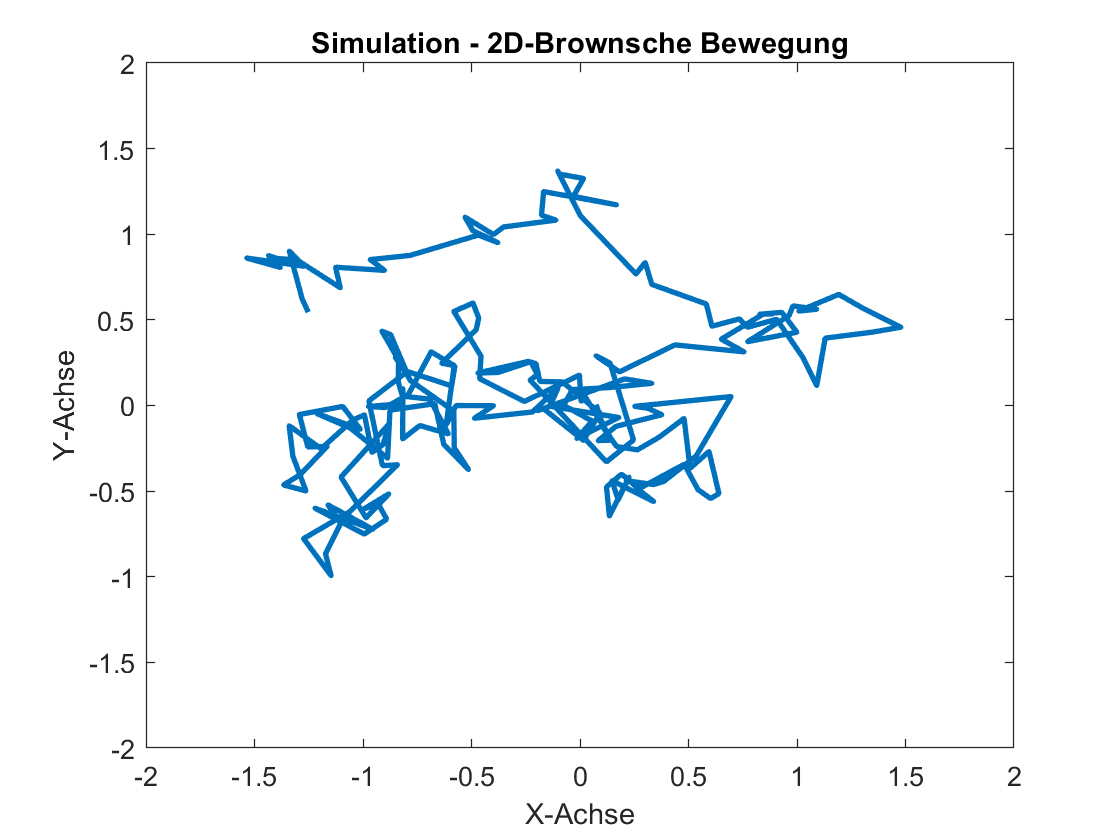
\includegraphics[width=\linewidth]{papers/brown/images/Brownische-Bewegung-Simuliert_2.png}
		\caption{Second subfigure}
	\end{minipage}
	\caption{Two subfigures side-by-side}
\end{figure}

